\documentclass[a4paper]{article}

%use the english line for english reports
%usepackage[english]{babel}
\usepackage[portuguese]{babel}
\usepackage[utf8]{inputenc}
\usepackage{indentfirst}
\usepackage{graphicx}
\usepackage{verbatim}
\usepackage[numbers,square, comma, sort&compress]{natbib}
\usepackage[top=4cm, bottom=3cm, left=3cm, right=3.5cm]{geometry}

\begin{document}

%\setlength{\textwidth}{16cm}
%\setlength{\textheight}{22cm}

\title{\Huge\textbf{Dominup em Prolog}\linebreak\linebreak\linebreak
\Large\textbf{Relatório Intercalar}\linebreak\linebreak
\linebreak\linebreak

\includegraphics[scale=0.1]{feup-logo.png}\linebreak\linebreak
\linebreak\linebreak
\Large{Mestrado Integrado em Engenharia Informática e Computação} \linebreak\linebreak
\Large{Programação em Lógica}\linebreak
}

\author{\textbf{Dominup4:}\\
Ângela Filipa Pereira Cardoso - up200204375 \\
Nuno Miguel Rainho Valente - up200204376 \\
\linebreak\linebreak \\
 \\ Faculdade de Engenharia da Universidade do Porto \\ Rua Roberto Frias, s\/n, 4200-465 Porto, Portugal \linebreak\linebreak\linebreak
\linebreak\linebreak\vspace{1cm}}

\maketitle
\thispagestyle{empty}

%************************************************************************************************
%************************************************************************************************

\newpage

%Todas as figuras devem ser referidas no texto. %\ref{fig:codigoFigura}
%
%%Exemplo de código para inserção de figuras
%%\begin{figure}[h!]
%%\begin{center}
%%escolher entre uma das seguintes três linhas:
%%\includegraphics[height=20cm,width=15cm]{path relativo da imagem}
%%\includegraphics[scale=0.5]{path relativo da imagem}
%%\includegraphics{path relativo da imagem}
%%\caption{legenda da figura}
%%\label{fig:codigoFigura}
%%\end{center}
%%\end{figure}
%
%
%\textit{Para escrever em itálico}
%\textbf{Para escrever em negrito}
%Para escrever em letra normal
%``Para escrever texto entre aspas''
%
%Para fazer parágrafo, deixar uma linha em branco.
%
%Como fazer bullet points:
%\begin{itemize}
	%\item Item1
	%\item Item2
%\end{itemize}
%
%Como enumerar itens:
%\begin{enumerate}
	%\item Item 1
	%\item Item 2
%\end{enumerate}
%
%\begin{quote}``Isto é uma citação''\end{quote}


%%%%%%%%%%%%%%%%%%%%%%%%%%
\section{O Jogo Dominup}

Dominup é uma variação do jogo Dominó para 2 a 4 jogadores, em que, tal como o nome sugere, é possível colocar peças em cima de outras.

No típico Dominó existem 28 peças duplas numeradas de 0 a 6, à semelhança das faces de um dado. Já no Dominup há 36 peças duplas numeradas de 0 a 7, usando códigos binários: o ponto no centro representa 1, o circulo pequeno representa 2 e o circulo grande representa 4, como se pode ver na figura~\ref{piece}. Este desenho das peças, juntamente com as regras do Dominup e de dois outros jogos, foram criadas por Néstor Romeral Andrés em 2014, sendo o conjunto publicado por nestorgames\footnote[1]{http://www.nestorgames.com}.

\begin{figure}[h!]
\begin{center}

\includegraphics[scale=0.5]{piece.jpg}
\caption{Exemplo da peça $3 \cdot 6$.}
\label{piece}
\end{center}
\end{figure}

Existem dois tipos de colocação de peças no Dominup:
\begin{itemize}
	\item subir - a peça é colocada em cima de duas peças adjacentes que estejam ao mesmo nível, de forma a que os números da peça colocada sejam iguais aos que ficam por baixo (um em cada peça de suporte), tal como mostra a figura~\ref{climb}.
	\item expandir - a peça é colocada na superfície de jogo, de forma a que fique adjacente e ortogonal a pelo menos uma peça já colocada, como, por exemplo, as duas peças já colocadas na figura~\ref{climb}.
\end{itemize}

\begin{figure}[h!]
\begin{center}
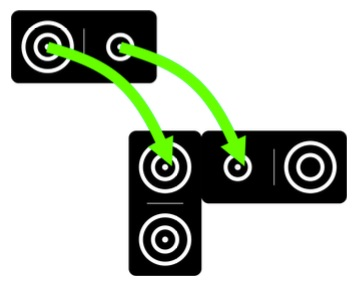
\includegraphics[scale=0.6]{climb.jpg}
\caption{Exemplo de um posicionamento a subir válido.}
\label{climb}
\end{center}
\end{figure}

Tal como no Dominó, as regras são relativamente simples. Começa-se por distribuir as peças aleatoriamente e de forma equilibrada pelos jogadores, mantendo a face voltada para baixo. 

O jogador com o duplo 7 inicia o jogo, colocando essa peça no centro da superfície de jogo e determinando a ordem dos restantes jogadores, que é dada pelo sentido contrário ao ponteiro dos relógios. 

Começando no segundo, cada jogador, na sua vez, realiza ambos os passos seguintes:
\begin{enumerate}
	\item Enquanto for possível, coloca peças a subir, podendo escolher a ordem em que o faz;
	\item Se ainda tiver alguma peça, coloca-a a expandir.
\end{enumerate}

Se, no final da sua vez, o jogador ficar sem peças, é declarado vencedor e o jogo termina. Alternativamente, os restantes jogadores podem continuar, de forma a determinar o segundo, terceiro e quarto lugares.

Na figura~\ref{example} pode ser observado um possível jogo de Dominup a decorrer.

\begin{figure}[h!]
\begin{center}
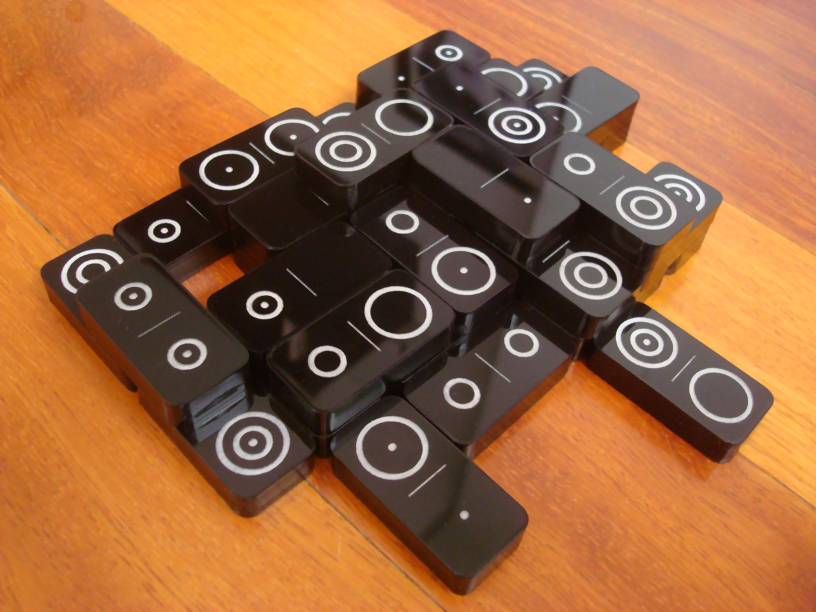
\includegraphics[scale=0.4]{example.jpg}
\caption{Exemplo de um jogo de Dominup.}
\label{example}
\end{center}
\end{figure}


%Descrever detalhadamente o jogo, a sua história e, principalmente, as suas regras.
%Devem ser incluidas imagens apropriadas para explicar o funcionamento do jogo.
%Devem ser incluidas as fontes de informação (e.g. URLs em rodapé).


%%%%%%%%%%%%%%%%%%%%%%%%%%
\section{Representação do Estado do Jogo}

O tabuleiro de jogo no Dominup é um quadriculado, cujo tamanho não deve limitar o posicionamento de peças a expandir. Uma vez que expansões sucessivas têm que ser feitas ortogonalmente, uma linha expansiva numa só direção ocupa $2 + 1 + 2 + 1 + \cdots$ quadrículas, assumindo que a primeira peça está colocada horizontalmente. Ao todo temos 36 peças, por isso seriam necessárias $2 * 18 + 18 = 54$ quadrículas para acomodar uma tal linha de expansão. Dado que a primeira peça é colocada no centro do tabuleiro, se a expansão fosse feita sempre no mesmo sentido, poderíamos ter que considerar um tabuleiro com 108 quadrículas de lado.

Uma análise mais cuidada das regras do jogo revela que as peças são preferencialmente colocadas a subir. De facto, em cada vez, um jogador coloca tantas peças a subir quanto possível e no máximo uma peça a expandir. Além disso, em geral não será boa estratégia para nenhum dos jogadores expandir sempre no mesmo sentido. Tendo em consideração as limitações de um computador, quer em termos de capacidade de processamento, quer em termos de tamanho do ecrã, decidimos considerar um tabuleiro quadriculado de lado 24. Desta forma, é possível colocar pelo menos 8 peças em cada um dos 4 sentidos a partir do centro do tabuleiro. Eventualmente, com a experiência, podemos decidir reduzir ou aumentar este tamanho. O ideal é que o tabuleiro nunca limite as jogadas, mantendo-se tão pequeno quanto possível para facilitar o processamento.

Sendo assim, o tabuleiro em Prolog é representado por uma lista $board$ de 24 linhas do tabuleiro. Por sua vez, cada linha é uma lista de 24 elementos, um para cada quadrícula. Cada elemento de uma linha é um termo complexo $half\_piece(number, level, cardinal)$ representando a meia peça de dominó lá colocada, com o seguinte significado:
\begin{itemize}
	\item $number$ é o número da meia peça;
	\item $level$ é o nível do tabuleiro em que a peça está colocada, 1 se for colocada em cima do tabuleiro, 2 se for colocada em cima dessa, etc;
	\item $cardinal$ é o ponto cardeal que indica a posição da outra metade da peça.
\end{itemize}
Assim, numa quadrícula vazia temos $half\_piece(\_, \_, \_)$. Quando é colocado o dominó duplo 7, teremos $half\_piece(7,1,e)$ e $half\_piece(7,1,o)$ em duas quadrículas adjacentes. Numa fase mais avançada pode ser colocado o dominó $2 \cdot 6$ no nível 3 na vertical com $half\_piece(2,3,n)$ e $half\_piece(6,3,s)$.

%Descrever a forma de representação do estado do tabuleiro (tipicamente uma lista de listas), com exemplificação em Prolog de posições iniciais do jogo, posições intermédias e finais, acompanhadas de imagens ilustrativas.


%%%%%%%%%%%%%%%%%%%%%%%%%%
\section{Visualização do Tabuleiro}

Descrever a forma de visualização do tabuleiro em modo de texto e o(s) predicado(s) Prolog construídos para o efeito.
Deve ser incluída pelo menos uma imagem correspondente ao output produzido pelo predicado de visualização.


%%%%%%%%%%%%%%%%%%%%%%%%%%
\section{Movimentos}

Elencar os movimentos (tipos de jogadas) possíveis e definir os cabeçalhos dos predicados que serão utilizados (ainda não precisam de estar implementados).


\end{document}
